\documentclass[11pt]{article}
\usepackage{../style/forage}

\newcommand{\emailfield}[2]{\textbf{\color{navy}#1}\quad #2\par}

\begin{document}
{\LARGE Market Advisory Email}\par\medskip
{\large Task 2 --- Navigating Live Market Dynamics \textperiodcentered\ Client:
Horizon Capital}\par
{\color{rulegray}\rule{\linewidth}{0.6pt}}\par\medskip

\begin{tcolorbox}[enhanced, colback=boxgray, frame hidden, arc=2mm,
    left=5mm, right=5mm, top=3mm, bottom=3mm]
\emailfield{To:}{Horizon Capital --- Investment Team}
\emailfield{From:}{Thiziri Amezza, Global Markets Sales \& Trading Analyst}
\emailfield{Subject:}{Sector update and recommended portfolio adjustments ---
Renewable Energy, Technology, Real Estate}
\end{tcolorbox}
\medskip

Dear Horizon Capital team,

Thank you for reaching out. Below is our read of the latest sector moves, what
they mean for your portfolio, and the three steps we recommend.

\heading{Key Trends Identified}
\begin{itemize}[leftmargin=1.5em, itemsep=3pt]
  \item \textbf{Renewable Energy: +2.5\%, positive sentiment, VIX 18.} The
  strongest move of the three, and sentiment supports it --- this looks like
  momentum, not noise.
  \item \textbf{Technology: \textminus1.2\%, neutral sentiment, VIX 22.} The
  only decline and the highest volatility. Falling prices, elevated volatility
  and no sentiment support make it the main risk in the portfolio today.
  \item \textbf{Real Estate: +0.8\%, stable sentiment, VIX 16.} The lowest
  volatility; it is doing its job as the portfolio's stabilizer.
  \item \textbf{Market context:} all three volatility readings sit in the
  15--25 ``normal fluctuation'' range. There is no market-wide stress, so this
  calls for targeted adjustments, not a defensive overhaul.
\end{itemize}

\heading{Portfolio Implications}
Your current allocation is Renewable Energy 40\%, Technology 30\%, Real Estate
20\%, Cash 10\%.
\begin{itemize}[leftmargin=1.5em, itemsep=3pt]
  \item On these moves the portfolio gained about \textbf{+0.8\%}: Renewable
  Energy added +1.0 point, Technology cost \textminus0.4 point.
  \item \textbf{Technology is 30\% of capital but about 39\% of the
  portfolio's volatility exposure.} This is exactly the ``excessive exposure to
  high-volatility assets'' you want to avoid.
  \item \textbf{Renewable Energy is driving returns}, but it is sensitive to
  policy and energy prices, so any increase should be measured.
  \item \textbf{Real Estate provides stability}; its main risk is a rise in
  interest rates and borrowing costs.
  \item \textbf{The 10\% cash reserve} is currently idle and can serve as a
  tool for agility.
\end{itemize}

\heading{Actionable Recommendations}
\begin{enumerate}[leftmargin=1.5em, itemsep=4pt]
  \item \textbf{Immediate --- reduce Technology from 30\% to 22\%.} This cuts
  exposure to the most volatile, underperforming sector while keeping a core
  position for when rates and the innovation cycle turn. Of the 8 points
  freed, 5 fund step~2 and 3 go to cash.
  \item \textbf{Immediate --- increase Renewable Energy from 40\% to 45\%, in
  two steps of 2.5\%} (this week and next). This captures the momentum while
  limiting timing risk. We suggest capping the sector at 45\% given its policy
  sensitivity, and reviewing it if its volatility rises above 25 or sentiment
  turns neutral.
  \item \textbf{Hold --- keep Real Estate at 20\%} as the portfolio anchor, and
  reassess if interest rates start to rise. Cash moves to 13\% as ``dry
  powder'': we would redeploy it into Technology once its volatility falls
  back below about 18 and sentiment turns positive, or keep it as a buffer if
  market volatility moves above 25.
\end{enumerate}

\begin{center}
\begin{tabular}{lrr}
  \toprule
  & \textbf{Current} & \textbf{Proposed} \\
  \midrule
  Renewable Energy & 40\% & 45\% \\
  Technology & 30\% & 22\% \\
  Real Estate & 20\% & 20\% \\
  Cash & 10\% & 13\% \\
  \midrule
  Weighted performance (this snapshot) & +0.80\% & +1.02\% \\
  Weighted volatility (VIX) & 17.0 & 16.1 \\
  Technology share of volatility & 39\% & 30\% \\
  \bottomrule
\end{tabular}
\end{center}

\textbf{How this fits your goals:} more capital in the strongest sector
supports growth; the smaller Technology position and the larger cash buffer
reduce volatility; and the staged entry and clear re-entry triggers keep you
agile as conditions change.

We are happy to execute on your approval. We will keep monitoring volatility,
sector sentiment and interest rates daily and will update you if any trigger
is reached.

\medskip
Best regards,\par\medskip
\textbf{Thiziri Amezza}\par
Global Markets Sales \& Trading Analyst

\newpage
{\Large\bfseries Appendix --- Supporting analysis}\par
{\small\color{gray}Not part of the email. All figures and tables are generated by
\texttt{analysis.ipynb}.}\par\medskip

\subheading{Figure 1 --- The live market snapshot}
\begin{center}
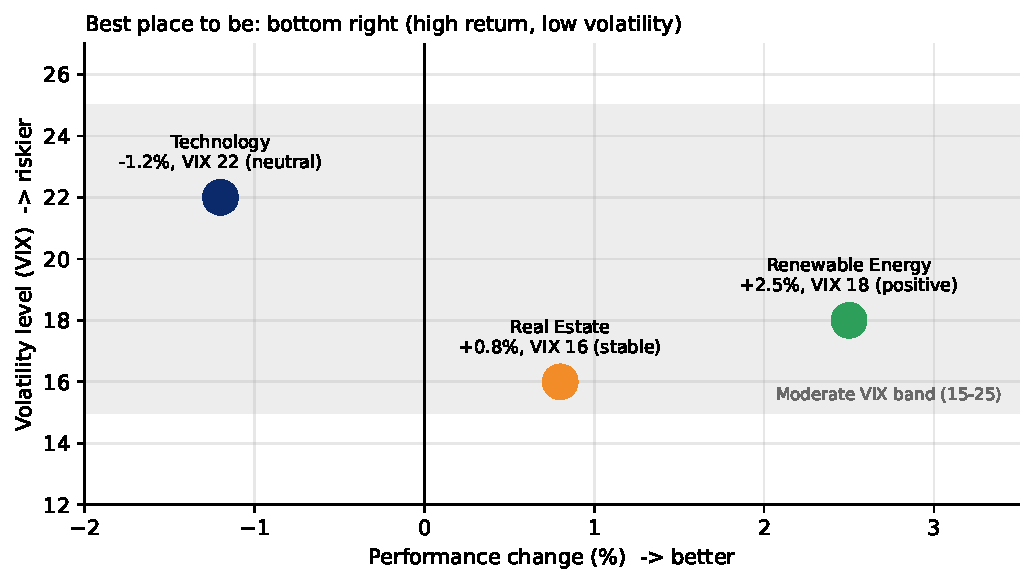
\includegraphics[width=0.78\linewidth]{figures/fig1_snapshot.pdf}
\end{center}

\subheading{Table 1 --- Allocations compared on the snapshot}
\begin{center}
\begin{tabular}{@{}lrrr@{}}
\toprule
 & \textbf{Current} & \textbf{Proposed} & \textbf{Forage example$^{*}$} \\
\midrule
Renewable Energy & 40\% & 45\% & 45\% \\
Technology & 30\% & 22\% & 25\% \\
Real Estate & 20\% & 20\% & 20\% \\
Cash & 10\% & 13\% & 10\% \\
\midrule
Weighted performance (this snapshot) & +0.80\% & +1.02\% & +0.98\% \\
Weighted volatility (VIX) & 17.0 & 16.1 & 16.8 \\
Technology share of volatility & 39\% & 30\% & 33\% \\
\bottomrule
\end{tabular}
\end{center}
{\footnotesize\color{gray}$^{*}$Forage's example answer: Renewable Energy +5
from cash, Technology \textminus5. It does not say where the 5 Technology
points go; read literally, the weights sum to 95\%. Shown here with those
points kept in cash.\par}

\subheading{Figure 2 --- Allocation and return vs.\ volatility}
\begin{center}
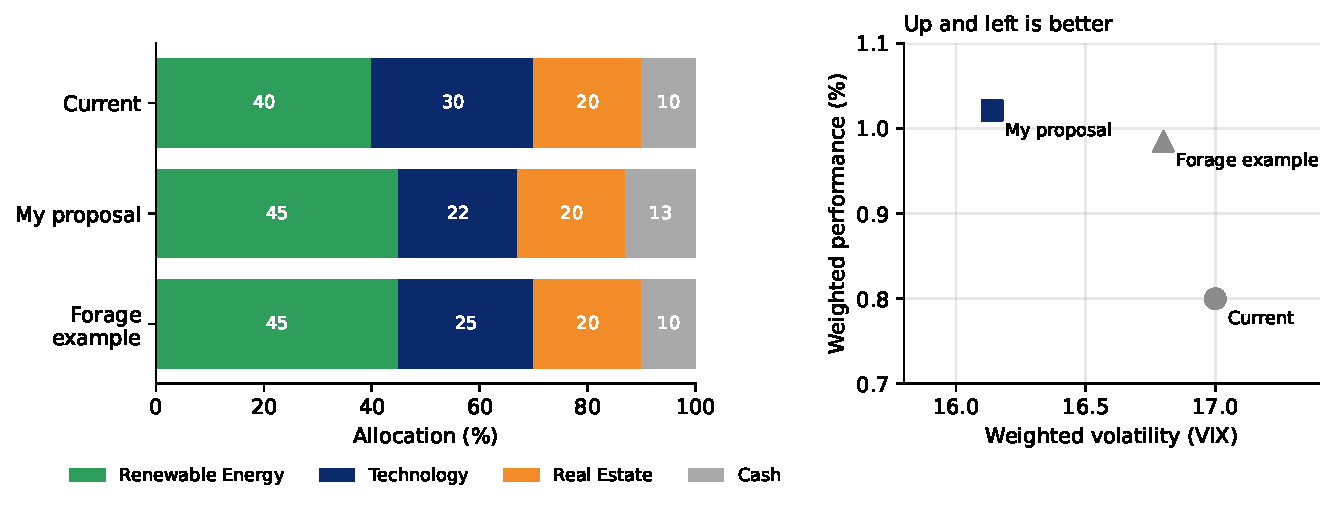
\includegraphics[width=\linewidth]{figures/fig2_allocation.pdf}
\end{center}

\subheading{Table 2 --- Stress test (portfolio impact of a shock)}
\begin{center}
\begin{tabular}{@{}lrrr@{}}
\toprule
Shock & \textbf{Current} & \textbf{Proposed} & \textbf{Forage example$^{*}$} \\
\midrule
Tech sell-off continues & \textminus{}1.50\% & \textminus{}1.10\% & \textminus{}1.25\% \\
Renewable policy shock & \textminus{}2.40\% & \textminus{}2.70\% & \textminus{}2.70\% \\
Rate rise (+50 bp) & \textminus{}1.70\% & \textminus{}1.51\% & \textminus{}1.60\% \\
\bottomrule
\end{tabular}
\end{center}
{\footnotesize\color{gray}Shocks are my own assumptions, based on the client's
key concerns. Tech sell-off: Technology \textminus5\%. Renewable policy shock:
Renewable Energy \textminus6\%. Rate rise: Renewable Energy \textminus1\%,
Technology \textminus3\%, Real Estate \textminus2\%. Cutting Technology helps
in two of the three shocks; the price of more Renewable Energy is a larger loss
in a policy shock, hence the 45\% cap, the staged entry and the review
trigger.\par}

\bigskip
{\color{rulegray}\rule{\linewidth}{0.4pt}}\par
{\footnotesize\color{gray}\textbf{Workings.} Data: Task 2 market snapshot
(sector performance, sentiment, VIX) and the Client Profile Reference Sheet.
Weighted performance $=\sum_i w_i\,r_i$, with cash at 0\% (current:
$0.40\times2.5+0.30\times(-1.2)+0.20\times0.8=0.80\%$). Weighted volatility
$=\sum_i w_i\,\mathrm{VIX}_i$ with cash at 0 (current: $7.2+6.6+3.2=17.0$);
Technology's share is $6.6/17.0\approx39\%$, falling to $4.84/16.14\approx30\%$
after the change. These figures describe the snapshot only and are not a
return forecast. VIX bands (below 15 low, 15--25 moderate, above 25 high) are
from the Live Market Indicators Guide.\par}
\end{document}
